\subsection{Causality and cyclic graphs}
\begin{frame}{Causality and cyclic graphs}
\label{sec:eberhardt}
\begin{columns}
\begin{column}{0.65\textwidth}
% Causal structure learning, where causal edges are inferred on graphs representing real systems, is often performed on DAGs, as described in a review by Heinze-Deml~et~al.~\cite{CausalLearningReview}. DAGs are too simple to use for biological networks where gene transcription products are taken into account. The only model in the review that is designed for cyclic graphs is BackShift, which is an extension of LLC~(Linear, Latents, Cyclic) described by Eberhardt~et~al.~\cite{EberhardtLLC}. Both methods are designed in pursuit of inferring network edges from node attributes observed under different interventions. The interventions are changes to nodes in the graph, which breaks all ingoing edges. In LLC it is assumed to be known which nodes have been intervened on, which is not assumed with BackShift. For knockout studies we know which nodes (genes) have been knocked out, so LLC is discussed here.
% We first assume a system of node values that are controlled linearly by the values from all parent nodes through discreet time steps~(\autoref{eq:eber_linear}).
Eberhardt et al.~\cite{CausalLearningReview}
\begin{subequations}
\label{eq:eber_linear}
\begin{align}
x_i (t) &=
    \sum_j b_{ij} x_j (t - 1) + e_i
\\
\label{eq:eber_linear.b}
\boldsymbol{x}(t) &=
    B \boldsymbol{x} (t - 1) + \boldsymbol{e}
=
    B \left( B \boldsymbol{x} (t - 2) + \boldsymbol{e} \right) + \boldsymbol{e} = ...
\\
&=
    B^t \boldsymbol{x}(0) + \sum_{i=0}^{t-1} B^i \boldsymbol{e}
\label{eq:eber_time.b}
\\
\lim_{t \rightarrow \infty} B^t &= 0
\quad,\quad
\lim_{t \rightarrow \infty} \sum_{i=0}^{t-1} B^i = \left( I - B \right)^{-1}
\qquad\qquad\qquad\text{\cite{Fisher1970}}
\label{eq:eber_converge}
\end{align}
\end{subequations}
% $e_i$ is added as a term to describe latent variables and noise. Latent variables are any hidden variables in the network not included in $\boldsymbol{x}(t)$.
% We can imagine how this generalizes to any time $t$ relative to the start time $t=0$~(\autoref{eq:eber_time}).
% Having cycles in the model means there can be infinite loops of regulation so to capture all regulation effect for cycles in the model $t$ has to tend to infinity. We first have to assume that $\boldsymbol{x}(t)$ converges for $t\rightarrow \infty$. A realistic system is not expected to diverge. Microorganism have exponential growth hindered only by outside factors that we are not considering in the model, but the growth is exponential due to unhindered cell division, but we assume that there is no exponentially increasing level of synthesis inside the cell, and we only model the workings inside a single cell. There is of course another option which is that $\boldsymbol{x}(t)$ fluctuates or in another way neither converges to an equilibrium nor diverges to infinity. Eberhardt~et~al. also considers this and proofs that the conditions for the model can be extended to accept semi-stable systems.
% Each of the two terms defining $\boldsymbol{x}(t)$~(\autoref{eq:eber_time.b}) are found without restriction on $\boldsymbol{x}(0)$ and $\boldsymbol{e}$ when $t$ tends to infinity~(\autoref{eq:eber_converge}):
% The equations hold when all eigenvalues $\lambda_k$ of $B$ satisfies $|\lambda_k| < 1$~\cite{Fisher1970}. The notation with indication of time is dropped when equilibrium is reached:
Equilibrium
\begin{subequations}
\label{eq:eber_simple}
\begin{align}
\lim_{t \rightarrow \infty} \boldsymbol{x}(t) = \boldsymbol{x} &=
    \left( I - B \right)^{-1} \boldsymbol{e}
\\
\left( I - B \right) \boldsymbol{x} &=
    \boldsymbol{e}
\\
\boldsymbol{x} &=
    B \boldsymbol{x} + \boldsymbol{e}
\end{align}
\end{subequations}
\end{column}
\begin{column}{0.35\textwidth}
\begin{figure}[ht]
    \centering
    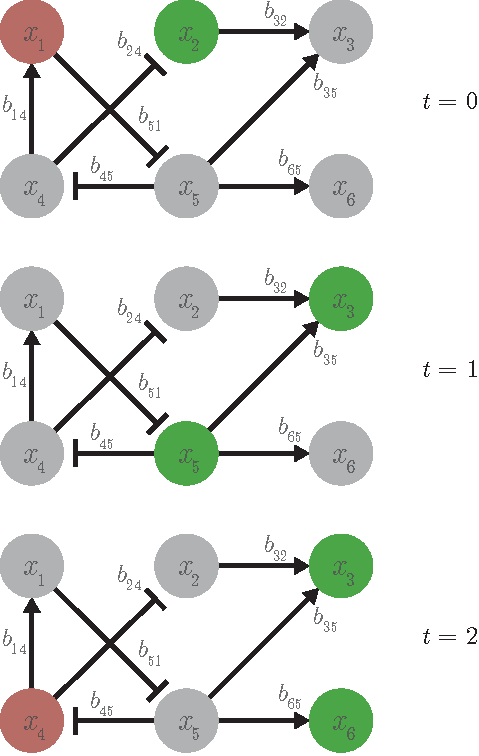
\includegraphics[width=.8\textwidth]{theory/fig/eberhardt.pdf}
    \caption{\textbf{Graph with constant edges.} \\ \textcolor{gray}{Gray} = 0, \textcolor{red!60!black}{red} < 0, \textcolor{green!45!black}{green} > 0.}
    \label{fig:eberhardt}
\end{figure}
\end{column}
\end{columns}
\end{frame}
\begin{frame}{Causality and cyclic graphs - Intervention}
\begin{columns}
\begin{column}{0.65\textwidth}
% We see that the convergence values are defined without referencing the node values at $t=0$ and the expression otherwise exactly matches~\autoref{eq:eber_linear.b}, except that taking a step forward or backward in time does not change the node values anymore.

% The diagonal of $B$ describes edges from nodes onto themselves, self-loops. These are unidentifiable from equilibrium data, since it is impossible to tell the difference between an node with a strong activator and a node with a weaker activator but a strong self-loop only based on steady-state gene expression levels. For this reason the diagonal of $B$ is always set to zeros. 

% The model is then expanded to include a concept of intervention of variables which in the context of biological network experiments is the equivalent of a knockout experiment of one or more genes. The intervention is the replacement of a node with a new value that follows standard Gaussian noise independent of the other variables in the network~(\autoref{eq:eber_intervention}).
Intervention
\begin{subequations}
\label{eq:eber_intervention}
\begin{align}
\boldsymbol{x}_k(t) &=
    U_k B \boldsymbol{x}_k(t-1) + U_k \boldsymbol{e} + \boldsymbol{c}_k
\\
\lim_{t \rightarrow \infty} \boldsymbol{x}_k(t) = \boldsymbol{x}_k &=
    (I - U_k B)^{-1} (U_k \boldsymbol{e} + \boldsymbol{c}_k)
\\
(I - U_k B) \boldsymbol{x}_k &=
    U_k \boldsymbol{e} + \boldsymbol{c}_k
\\
\label{eq:eber_intervention.d}
\boldsymbol{x}_k &=
    U_k B \boldsymbol{x}_k + U_k \boldsymbol{e} + \boldsymbol{c}_k
\end{align}
\end{subequations}
\end{column}
\begin{column}{0.35\textwidth}
\begin{figure}
    \centering
    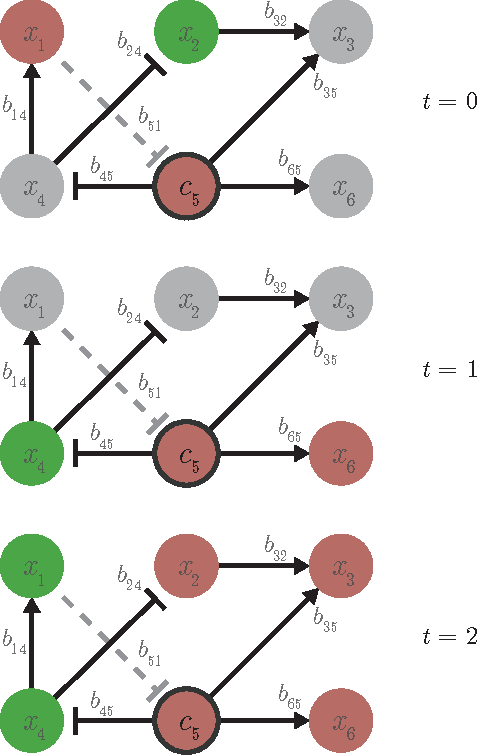
\includegraphics[width=.8\textwidth]{theory/fig/eberhardt_intervention.pdf}
    \caption{\textbf{Intervention on $x_5$.} \\ \textcolor{gray}{Gray} = 0, \textcolor{red!60!black}{red} < 0, \textcolor{green!45!black}{green} > 0.}
    \label{fig:intervention}
\end{figure}
\end{column}
\end{columns}
\end{frame}

\begin{frame}{Causality and cyclic graphs - $E[\boldsymbol{x}_k]$, covariance, and variable separation}
% The noise is given in $\boldsymbol{c}_k$ for the $k$-th experimental setup, where every value is zero except at the indexes of intervened nodes in experimental setup $k$. We refer to $k$ as an experimental setup rather than simply as an experiment to make it clear that the $k$-th experimental setup can be repeated multiple times, creating multiple observations of $\boldsymbol{x}_k$. The effect of other nodes onto the intervened variable is completely removed. 
% This makes sense in terms of a knockout where a removed gene will no longer be regulated by TFs. This is modelled using $U_k$ which is a diagonal matrix of ones, except at the indexes of intervened variables in experiment~$k$, where it has a value of zero. The result is the complete removal of the corresponding rows of $B$ and elements of $\boldsymbol{e}$. 
% A covariance matrix can be estimated if there are multiple observations for each experiment setup~$k$~(\autoref{eq:eber_cov}).
Expectation and covariance
\begin{subequations}
\label{eq:eber_cov}
\begin{align}
E[\boldsymbol{x}_k] &= (I-U_kB) ^{-1} \mu_{\boldsymbol{c}_k}
\\
\Sigma_{\boldsymbol{x}_k}
&=
\E \left[(\boldsymbol{x}_k - \E[\boldsymbol{x}_k] )(\boldsymbol{x}_k - \E[\boldsymbol{x}_k])^\trans \right]
\\
&= (I-U_kB)^{-1} E\left[ (U_k\boldsymbol{e}_k + \boldsymbol{c}_k - \mu_{\boldsymbol{c}_k})(U_k\boldsymbol{e}_k + \boldsymbol{c}_k - \mu_{\boldsymbol{c}_k})^\trans \right] (I-U_kB)^{-\trans}
\\
&= (I-U_kB)^{-1} (\Sigma_{\boldsymbol{c}_k} + U_k\Sigma_{\boldsymbol{e}} U_k) (I-U_kB)^{-\trans}
\end{align}
\end{subequations}
% Where $\mu_{\boldsymbol{c}_k}$ is the expected value of $\boldsymbol{c}_k$, and $\Sigma_{\boldsymbol{x}_k}$ is the covariance matrix of $\boldsymbol{x}_k$. The interesting parts of the covariance matrix are the entries describing covariance between the intervened variables and the passively observed variables. Since it is assumed that no variable has an effect onto intervened variables it can be possible to describe the observed covariance as more than just an undirected covariance edge between the two nodes but instead as a directed edge of causality from the intervened to the non-intervened.
% We denote the elements of vectors and matrices with subscript $\mathcal{J}_k$, $\mathcal{U}_k$, and $\mathcal{V}$ to refer to indexes for nodes intervened on in experimental setup $k$, passively observed in experimental setup $k$ and indexes of all nodes, respectively. We split our expression for $\boldsymbol{x}_k$ from \autoref{eq:eber_intervention.d} into expressions for intervened and non-intervened variables~(\autoref{eq:JU}).
Separating intervened ($\boldsymbol{x}_{\mathcal{J}_k}$) and passively observed ($\boldsymbol{x}_{\mathcal{U}_k}$) variables
\begin{subequations}
\label{eq:JU}
\begin{align}
\boldsymbol{x}_{\mathcal{J}_k} &= \boldsymbol{c}_{\mathcal{J}_k}
\\
\boldsymbol{x}_{\mathcal{U}_k} &= B_{\mathcal{U}_k\mathcal{V}} \boldsymbol{x}_k + \boldsymbol{e}_{\mathcal{U}_k}
\\
&= B_{\mathcal{U}_k\mathcal{U}_k} \boldsymbol{x}_{\mathcal{U}_k} + B_{\mathcal{U}_k\mathcal{J}_k} \boldsymbol{x}_{\mathcal{J}_k} + \boldsymbol{e}_{\mathcal{U}_k}
\\
(I - B_{\mathcal{U}_k\mathcal{U}_k}) \boldsymbol{x}_{\mathcal{U}_k} &=
B_{\mathcal{U}_k\mathcal{J}_k}\boldsymbol{x}_{\mathcal{J}_k} + \boldsymbol{e}_{\mathcal{U}_k}
\\
\boldsymbol{x}_{\mathcal{U}_k} &=
(I - B_{\mathcal{U}_k\mathcal{U}_k})^{-1}(B_{\mathcal{U}_k\mathcal{J}_k}\boldsymbol{x}_{\mathcal{J}_k} + \boldsymbol{e}_{\mathcal{U}_k})
\end{align}
\end{subequations}
\end{frame}

\begin{frame}{Causality and cyclic graphs - Covariance between $\boldsymbol{x}_{\mathcal{J}_k}$ and $\boldsymbol{x}_{\mathcal{U}_k}$}
% The covariance between $\boldsymbol{x}_{\mathcal{J}_k}$ and $\boldsymbol{x}_{\mathcal{U}_k}$ can then be described~(\autoref{eq:causal_cov}).
Covariance between intervened ($\boldsymbol{x}_{\mathcal{J}_k}$) and passively observed ($\boldsymbol{x}_{\mathcal{U}_k}$) variables
\begin{subequations}
\label{eq:causal_cov}
\begin{align}
(\Sigma_{\boldsymbol{x}_k})_{\mathcal{J}_k\mathcal{U}_k} &=
\E \left[ (\boldsymbol{x}_{\mathcal{J}_k} - \E[\boldsymbol{x}_{\mathcal{J}_k}])
(\boldsymbol{x}_{\mathcal{U}_k} - \E[\boldsymbol{x}_{\mathcal{U}_k}])^\trans \right]
\\
&= \E \left[
(\boldsymbol{x}_{\mathcal{J}_k} - \E[\boldsymbol{x}_{\mathcal{J}_k}])
(B_{\mathcal{U}_k\mathcal{J}_k} (\boldsymbol{x}_{\mathcal{J}_k} - \E[\boldsymbol{x}_{\mathcal{J}_k}]))^\trans
\right]
(I - B_{\mathcal{U}_k\mathcal{U}_k})^{-\trans}
\\
&= (\Sigma_{\boldsymbol{c}_k})_{\mathcal{J}_k\mathcal{J}_k} B^\trans_{\mathcal{U}_k\mathcal{J}_k} (I - B_{\mathcal{U}_k\mathcal{U}_k})^{-\trans}
\end{align}
\end{subequations}
% Eberhardt~et~al. deals with what they call canonical experiments to simplify notation where each element in $\boldsymbol{c}_k$ is uncorrelated with zero mean and unit variance. From this and the symmetry of covariance matrices we get expression for covariance between intervened and passively observed that only depend on entries of $B$~(\autoref{eq:eberhardt_cov}). Matrix $T_{\boldsymbol{x}_k}$ is also introduced here.
Using i.i.d. interventions $\boldsymbol{c}_k$
\begin{subequations}
\label{eq:eberhardt_cov}
\begin{align}
(\Sigma_{\boldsymbol{c}_k})_{\mathcal{J}_k\mathcal{J}_k} &= I
\\
(\Sigma_{\boldsymbol{x}_k})_{\mathcal{J}_k\mathcal{U}_k} &= B^\trans_{\mathcal{U}_k\mathcal{J}_k} (I - B_{\mathcal{U}_k\mathcal{U}_k})^{-\trans}
= T_{\boldsymbol{x}_k}^\trans
\\
(\Sigma_{\boldsymbol{x}_k})_{\mathcal{U}_k\mathcal{J}_k} &=
T_{\boldsymbol{x}_k} =
(I - B_{\mathcal{U}_k\mathcal{U}_k})^{-1} 
B_{\mathcal{U}_k\mathcal{J}_k} 
\end{align}
\end{subequations}
\end{frame}

\begin{frame}{Causality and cyclic graphs - Experimental effect}
% A concept of the overall effect from node $x_i$ to $x_u$, referred to as "experimental effect", is introduced~(\autoref{eq:experimental_effect}). It should be read as the total experimental effect from $x_i$ on $x_u$ given the conditions where $\mathcal{J}_k$ refers to the indexes of intervened variables in experimental setup $k$.
Total effect from $x_i$ to $x_u$ is sum of all directed paths
\begin{subequations}
\label{eq:experimental_effect}
\begin{align}
t(x_i \rightsquigarrow x_u || \mathcal{J}_k) &= \sum_{p \in \mathcal{P}(x_i \rightsquigarrow x_u || \mathcal{J}_k)} \prod_{(x_l \rightarrow x_m) \in p} b_{ml}
\\
\label{eq:t_to_b}
&= b_{ui} + \sum_{x_j \in \mathcal{U}_k \setminus \{x_u\}} t(x_i \rightsquigarrow x_j || \mathcal{J}_k) b_{uj}
\end{align}
\end{subequations}

% It is defined as summing the effects from each path from $x_i$ to $x_u$, where the effect along a given path is simply the product over all edge values $b_{ml}$ along that path. Since the graph has cycles there can be an infinite number of paths connecting $x_i$ and $x_u$. 

% In appendix C of 
Eberhardt~et~al.~\cite{EberhardtLLCdetail} proves
\begin{equation}
    t(x_i \rightsquigarrow x_u || \mathcal{J}_k) = (T_{\boldsymbol{x}_k})_{\{x_u\}\{x_i\}}
\end{equation}

%, which means that the experimental effect is equal to the element $u,i$ of the covariance matrix in the case where $x_i$ is intervened upon and $x_u$ is not. The empirical covariance matrix of observed variables can be used as an approximation of the true covariance matrix and thereby used for finding $t(x_i \rightsquigarrow x_u || \mathcal{J}_k)$ for different indexes of $i$ and $u$. As formulated in \autoref{eq:t_to_b} the values of $t(x_i \rightsquigarrow x_u || \mathcal{J}_k)$ are related to the values of $B$ where multiple observations can form a linear system of equations to solve for $B$.
% The resulting LLC algorithm does exactly this.
LLC (Linear, Latent, Cyclic) algorithm overview
\begin{equation}
\Sigma_{\boldsymbol{x}_k}
\rightarrow
T_{\boldsymbol{x}_k}
\rightarrow
t(x_i \rightsquigarrow x_u || \mathcal{J}_k)
\rightarrow
B
\end{equation}
% An issue arises when the covariance matrix cannot be estimated as is the case if there is only a single observation of $\boldsymbol{x}_k$ for each experimental setup $k$. $t(x_i \rightsquigarrow x_u || \mathcal{J}_k)$ is considered a regression coefficient when regressing $x_u$ over the only manipulated variable $x_i$, which means it is calculated as a linear regression coefficient where each observation is treated as the expected value~(\autoref{eq:t_regress}).
If covariance is unknown
\begin{equation}
\label{eq:t_regress}
t(x_i \rightsquigarrow x_u || \{x_i\}) \cdot x_i = x_u
\implies
t(x_i \rightsquigarrow x_u || \{x_i\}) = \frac{x_u}{x_i}
\end{equation}

% LLC is available as \texttt{R}-code, which was used for the $B$-method introduced in~\autoref{sec:equilibrium_inference}.


\end{frame}

